\documentclass[fleqn, letterpaper]{amsart}
%\documentclass[letterpaper]{tufte-handout}
%\usepackage{times}
\usepackage{amsmath}
\usepackage{amssymb}
\usepackage{graphicx}
\usepackage{booktabs}
\usepackage{multirow}
%\usepackage{listings}
\usepackage{epstopdf}
\usepackage{bm}
%\usepackage[left=1in]{geometry}

\newcommand{\R}{\mathcal{R}}
\newcommand{\E}{\text{E}}
\newcommand{\p}{p_{XY}}
\newcommand{\T}{^\text{T}}
\newcommand{\y}{\mathbf{y}}
\newcommand{\z}{\mathbf{z}}
\newcommand{\I}{\mathbf{I}}
\newcommand{\HH}{\mathbf{H}}
\newcommand{\A}{\mathbf{A}}
\newcommand{\GG}{\mathbf{G}}
\newcommand{\vecy}{\mathbf{y}}
\newcommand{\uu}{\mathbf{u}}
\newcommand{\cyy}{\mathbf{C}_{yy}}
\newcommand{\cyz}{\mathbf{C}_{yz}}
\newcommand{\czz}{\mathbf{C}_{zz}}
\newcommand{\cuu}{\mathbf{C}_{uu}}
\newcommand{\cvv}{\mathbf{C}_{vv}}
\newcommand{\cpp}{\mathbf{C}_{\psi\psi}}
\renewcommand{\arraystretch}{1.5}
\renewcommand{\vec}[1]{\mathrm{#1}}

\title{Course Project --- ENCE689E Spring 2014}
\author{David Prentiss}

\begin{document}
\maketitle

\section{Project Summary}

The Famine Early Warning System Network (FEWSNET) project is a federally funded effort to monitor regional and global economies, food, and climate in order to provide advanced warning of humanitarian, food related disasters.
Among the many FEWSNET tools is a model of pastoral herds. This model\cite{fewsnet} is an aid to the analysis of food security in regions where pastoral livelihoods are prevalent. While it sees wide adoption among food security analysts, its statistical properties are not well investigated.
Furthermore it may be possible to enhance this model with adaptive filtering techniques.
This work investigates the model's general charachteristics and assess the skill of the Ensemble Kalman Filter (EnKF) for data assimilation in a synthetic twin experiment.

\section{Herd Dynamics Model}

The herd dynamics model predicts the size and demographic features of a hypothetical herd from season to season based on the previous season's rainfall amount and quality.
These demographic features are sub--groups related to sex and reproductive capacity where individuals are categorized as either adult female, newborn, young female, or young male.
As such, the state of the herd at each season $t$, where $t$ is an index of sequential seasons is captured by the state vector $\vecy_t$.
The elements of $\vecy_t$ are the head--counts of individuals in each sub--group at the beginning of season $t$.
\begin{align}
y_{\text{AF}}^{t+1} &= [y_{\text{AF}}^t + y_{\text{YF}}^t - f_{\text{SF}}^ty_{\text{AF}}^t - f_{\text{MM}}^ty_{\text{AF}}^t]w_{\text{AF}}\\
y_{\text{NB}}^{t+1} &= [f_{\text{C}}^ty_{\text{AF}}^t]w_{\text{NB}}\\
y_{\text{YF}}^{t+1} &= [0.5(y_{\text{NB}}^t - f_{\text{MI}}^ty_{\text{NB}}^t) - f_{\text{MM}}^ty_{\text{YF}}^t]w_{\text{YF}}\\
y_{\text{YM}}^{t+1} &= [y_{\text{YM}}^t + y_{\text{NB}}^t - y_{\text{YF}}^{t+1} - f_{\text{SM}}^ty_{\text{YM}}^t - f_{\text{MM}}^ty_{\text{YM}}^t]w_{\text{YM}}
\end{align}
where $f_{\text{C}}^t$, $f_{\text{SM}}^t$, $f_{\text{SF}}$, $f_{\text{MM}}$, and $f_{\text{MI}}$ are the rates of conception, male sales, female sales, mature mortality, and immature mortality respectively and
$w_{\text{C}}^t$, $w_{\text{SM}}^t$, $w_{\text{SF}}$, $w_{\text{MM}}$, and $w_{\text{MI}}$
are multiplicative model error.
The rate functions have been determined empirically and are illustrated in Figure \ref{rferels}.

For model error $w$ the following properties are adopted:
\[w\sim\ln\mathcal{N}(\mu,\sigma), \bar{w}=1, \sigma_w^2 = 0.001\]
Multiplicative, lognormal error is chosen to avoid negative values.
However, the choice means that data assimilation techniques that assume a Guassian distribution for random variables, such as the Kalman Filter, are excluded.
\begin{figure}
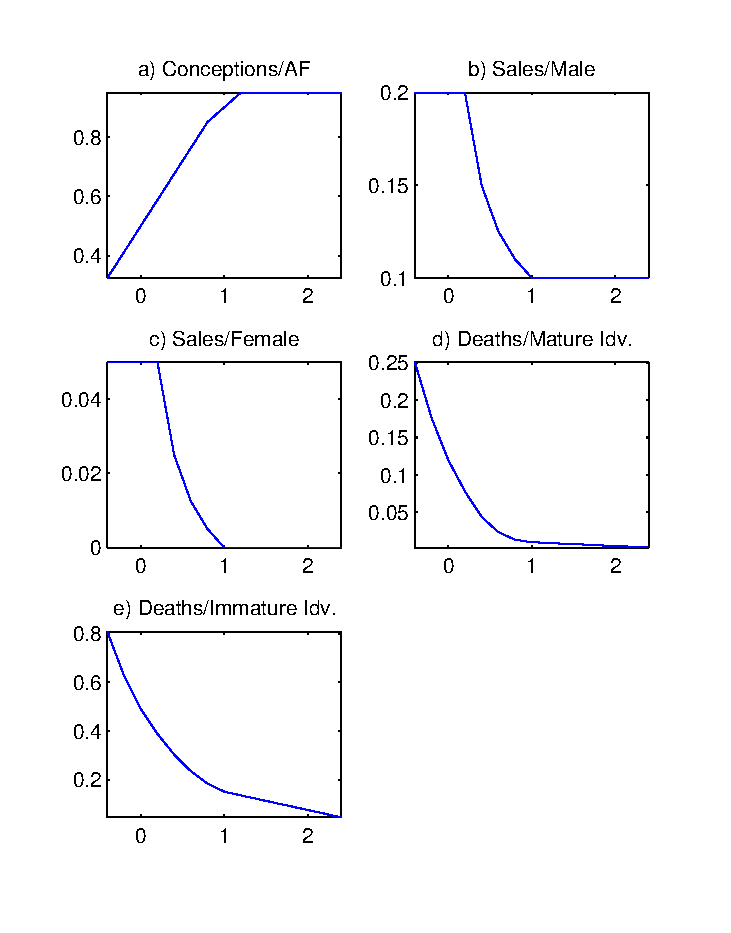
\includegraphics[width=1.0\textwidth]{refrel}
\caption{Herd Dynamic Rates. For each relationship, the y--axis represents the fraction of the relevent demographic group subject to change due to rainfall. The x--axis represents the current--season fraction of the regional average rainfall. Note: the negative values present in the dataset are undefined in the current interpretation and, as such, are not used.}
\label{rferels}
\end{figure}

Measurements of the system are taken for newborns (state two) only. The measurement model $H$ then is
\[H = (0\ 1\ 0\ 0)^T.\]

\section{General Characteristics}
The herd dynamics model is unproven and under--analyzed. In order to asses the efficacy of data assimilation techniques, it will first be useful to account for model behavior in general. 
To that end, the following items are considered to judge the model's general dynamic characteristics and sensitivities. 

\subsection{General tendencies vis--a--vis damped and un--damped dynamics}
A variety of constant forcing values and initial conditions were modeled to determine any thresholds between stable and unstable behavior.
See Figures \ref{general0}, \ref{rgeneral1}, and \ref{rgeneral10}.
From the figures it may be seen that the model achieves some stability during the modeled 40--season period when rainfall is constant near \%10 of the regional average. For rainfall amounts less (more) than this, the model tends to zero (exponetial growth). In general we expect a drought to cause the herd to shrink. Furthermore, exponetial growth is expected of populations that do not experience resource shortages. However, stable behavior at the observed level suggests that the model overvalues rainfall and does not account for at least one other resource limitation. Otherwise, unchecked herd growth would occationally be experienced in the field. 
\begin{figure}
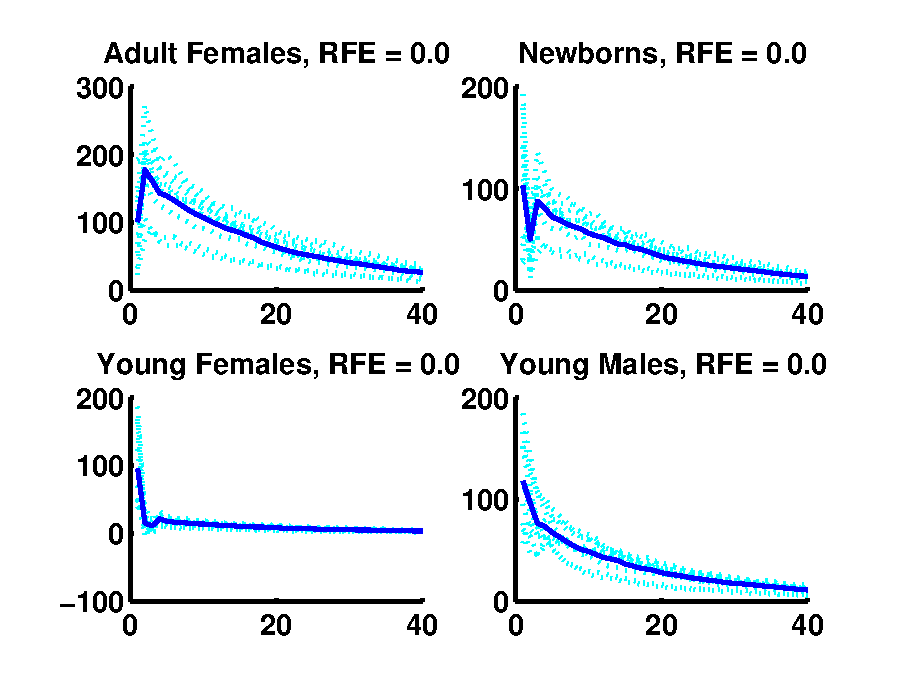
\includegraphics[width=\textwidth]{general0}
\label{general0}
\caption{Ten-member ensemble with consecutive seasons of zero rainfall.}
\end{figure}
\begin{figure}
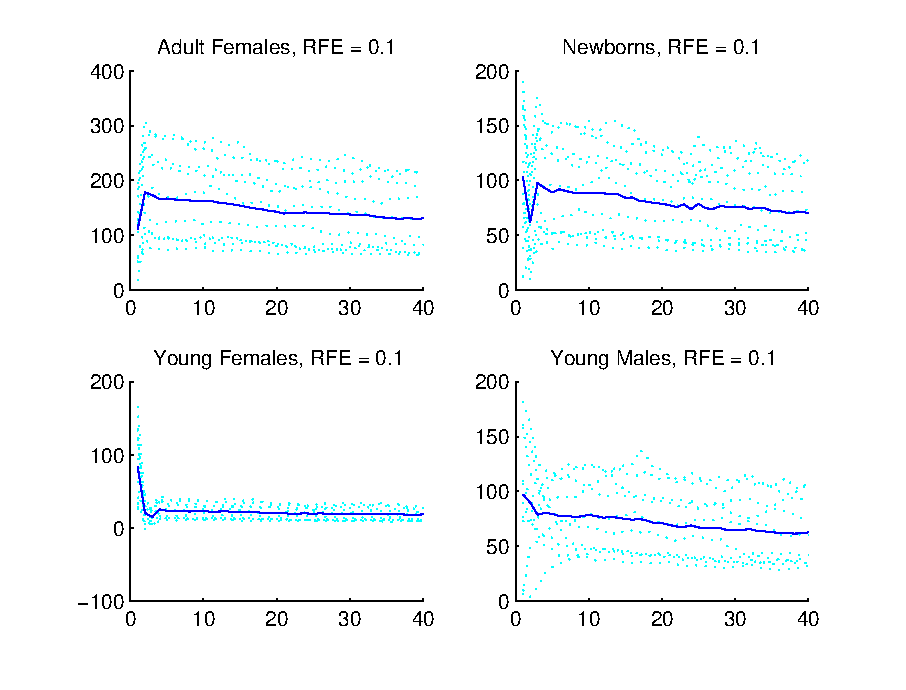
\includegraphics[width=\textwidth]{rgeneral1}
\label{rgeneral1}
\caption{Ten-member ensemble with consecutive seasons of rainfall at \%10 of regional average.}
\end{figure}
\begin{figure}
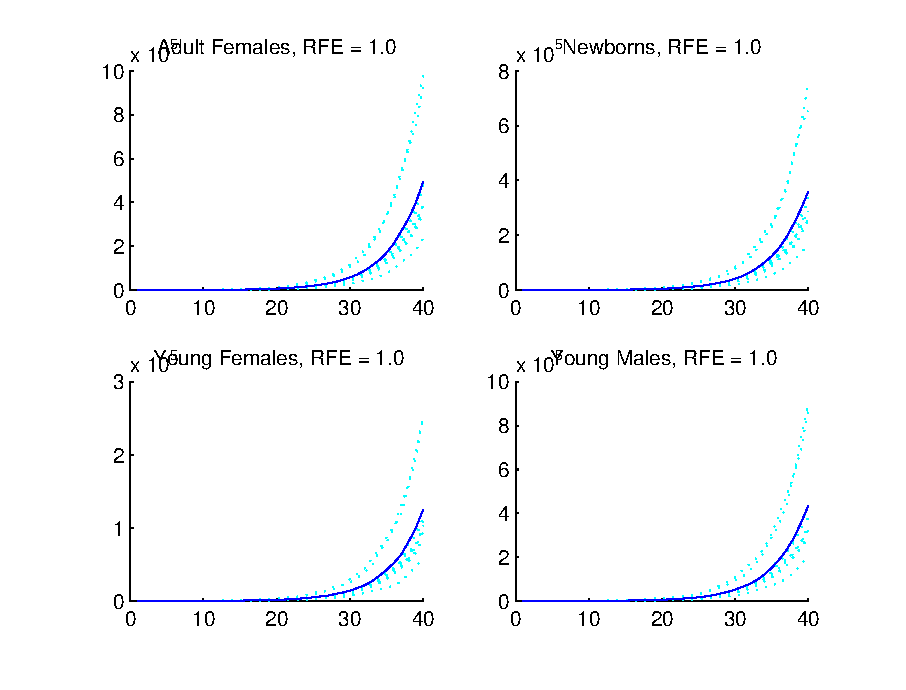
\includegraphics[width=\textwidth]{rgeneral10}
\label{rgeneral10}
\caption{Ten-member ensemble with consecutive seasons of rainfall at \%100 of regional average.}
\end{figure}

\subsection{Sensitivity to initial herd size and initial herd demographics}
Randomly chosen proportions of demographic sub--groups of herds with a fixed size were compared. As seen in Figure \ref{relprop}, the herd proportions quickly stabalize for time-invariant forcings. This result is expected given that for fixed forcings the rates of change are constant.
\begin{figure}
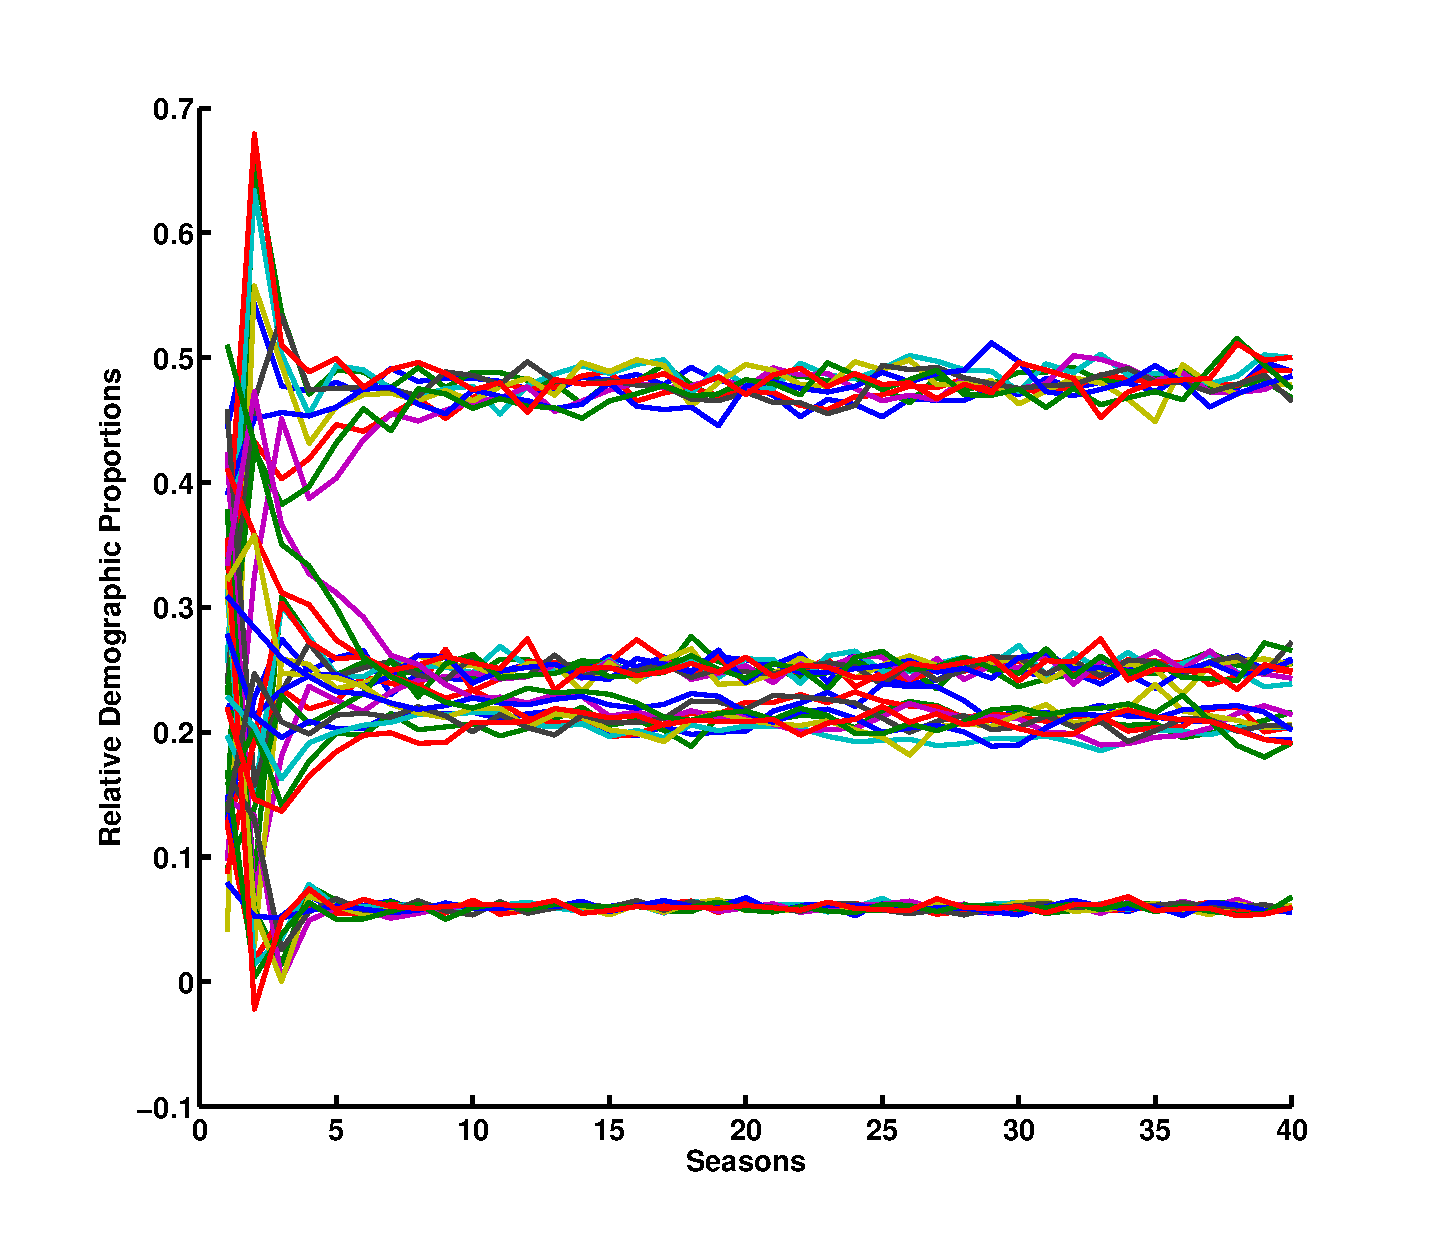
\includegraphics[width=0.9\textwidth]{relprop}
\caption{Relative Proportions of herd demographic--subgroups. For constant rainfall, herd proportions quickly stabalize.}
\label{relprop}
\end{figure}

\section{Data Assimilation}
The model, in its current form, is linear and little is know about its error characteristics.
As it stands, a different choice of error characteristics would allow the use of the  standard Kalman Filter for data assimilation under a Gaussian error assumption.
However, given that biological systems are often nonlinear and that the forcings are base on precipitation amounts and timings, both the linear dynamic and Gaussian assumptions may, after future updates to the model, be inappropriate.  As such, the skill of the EnKF is analysed. 

\subsection{Synthetic Truth}
To test the skill of the EnKF, the following synthetic truth was generated. An initial heard size and proportion was assumed with
\[\vecy_0 = (50\ 10\ 10\ 5)^T.\]
Also, 40 seasons of synthetic forcing were generated. The generation heuristic and initial conditions were chosen to simulate progressivly worsening drought conditions. See Figure \ref{forcing}.
Synthetic measurement were generated with a lognormal distribution with mean 0 and variance 0.001. 
\begin{figure}
\includegraphics[width=0.9\textwidth]{rforcing}
\label{forcing}
\caption{Synthetic forcing time series.}
\end{figure}
Running the open loop model for the generated initial conditions and forcings results in the synthetic truth time--series illustrated in Figure \ref{rtruth}.
\begin{figure}
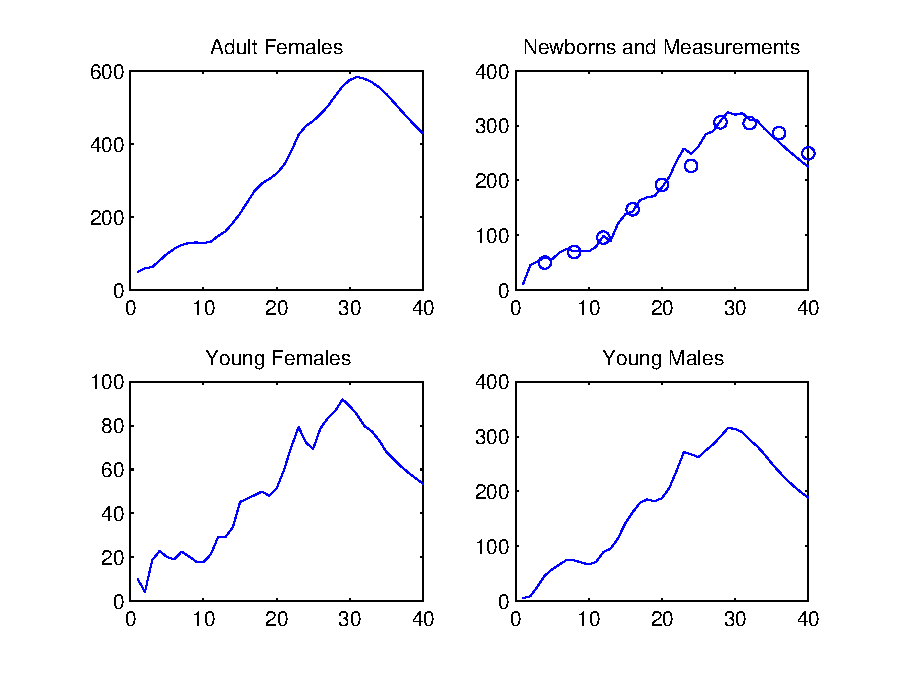
\includegraphics[width=0.9\textwidth]{rtruth}
\label{rtruth}
\caption{Synthetic truth time series.}
\end{figure}

\subsection{Recovery of initial conditions}
To assess the skill of the EnKF for recovery of initial conditions. A 100--member ensemble was generated with a uniform uncorrelated distribution, $y_0\sim\mathcal{U}(0,200)$.
The resulting ensemble had a mean of $(95\ 94\ 101\ 98)^T$ and covariance
\[\left(\begin{array}{cccc} 3345.0 & -515.0 & 220.6 & -144.6\\ -515.0 & 2995.0 & -665.7 & -53.02\\ 220.6 & -665.7 & 3431.0 & 72.85\\ -144.6 & -53.02 & 72.85 & 3061.0 \end{array}\right).\]
The results of the open loop are illustrated in Figure \ref{ol} and that of the EnKF in Figure \ref{kf}. The EnKF shows marked improvement in correcting for incorrect initial conditions. The comparison is listed in Table \ref{initcomp}.

\begin{figure}
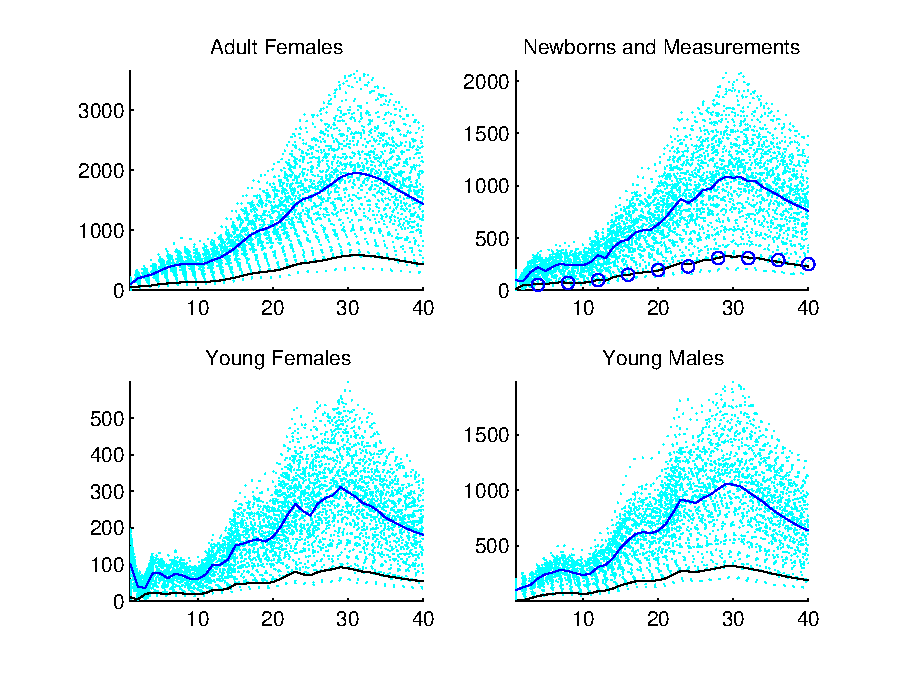
\includegraphics[width=0.9\textwidth]{ropenloop}
\label{ol}
\caption{Open loop results for a 100--member ensemble}
\end{figure}
\begin{figure}
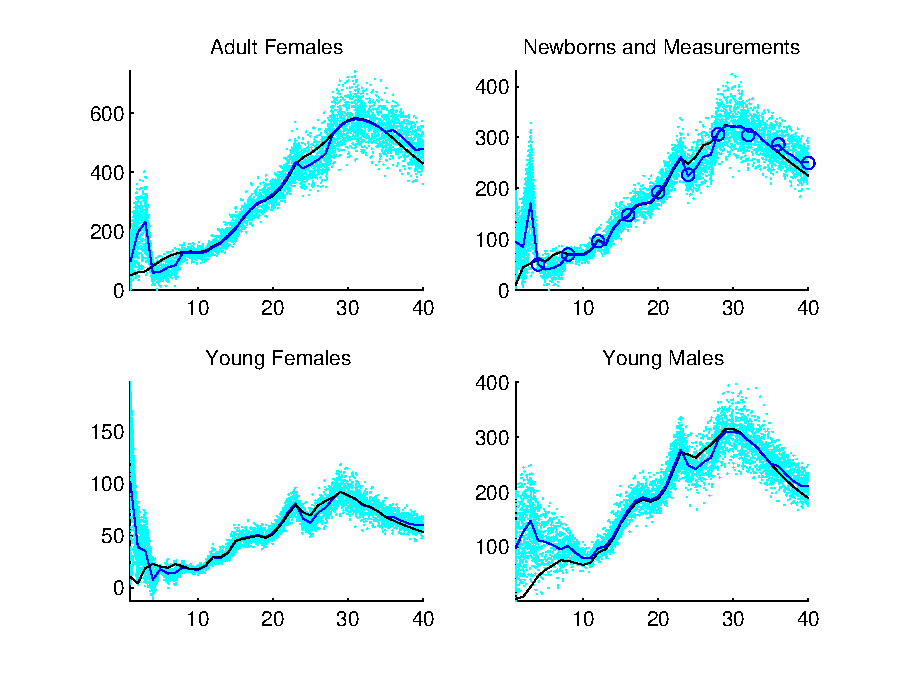
\includegraphics[width=0.9\textwidth]{kf}
\label{kf}
\caption{EnKF results for a 100--member ensemble}
\end{figure}
\begin{table}
\begin{tabular}{rrr}
& Bias & RMSE \\
\hline
Open loop & 441.2 & 565.2 \\
EnKF & 6.5 & 31.1
\end{tabular}
\label{initcomp}
\caption{Skill of open loop vs. EnKF}
\end{table}

\subsection{Sensitivity of skill to ensemble size}
The synthetic experiment was repeated for ensemble sizes of 10 and 1000. The comparison between the open loop and EnKF is tabultated in Table \ref{ensize}. The model showed constistant results across the range of ensemble sizes suggesting the model depends heavily on the measurements. This result is expected for a model with errer an order of magnitude higher than the measurement.
\begin{table}
\begin{tabular}{rrrr}
Ensemble members & 10 & 100 & 1000 \\
\hline
Bias & 10.5 & 6.5 & 6.5 \\
RMSE & 36.3 & 31.1 & 31.7
\end{tabular}
\label{ensize}
\caption{Skill for various ensemble sizes}
\end{table}

\subsection{Sensitivity of skill to model error variance}
The synthetic experiment was repeated for multiple values of the model error variance. The results are tabultated in Table \ref{error}. The model performed slightly worse for higher values of model error, as expected.
\begin{table}
\begin{tabular}{rrrr}
Model Error Variance & 0.001 & 0.01 & 0.1 \\
\hline
Bias & 6.5 & 7.2 & 9.7\\
RMSE & 31.1 & 30.9 & 40.7
\end{tabular}
\caption{Skill for various model error variances}
\label{error}
\end{table}


%\begin{figure}
%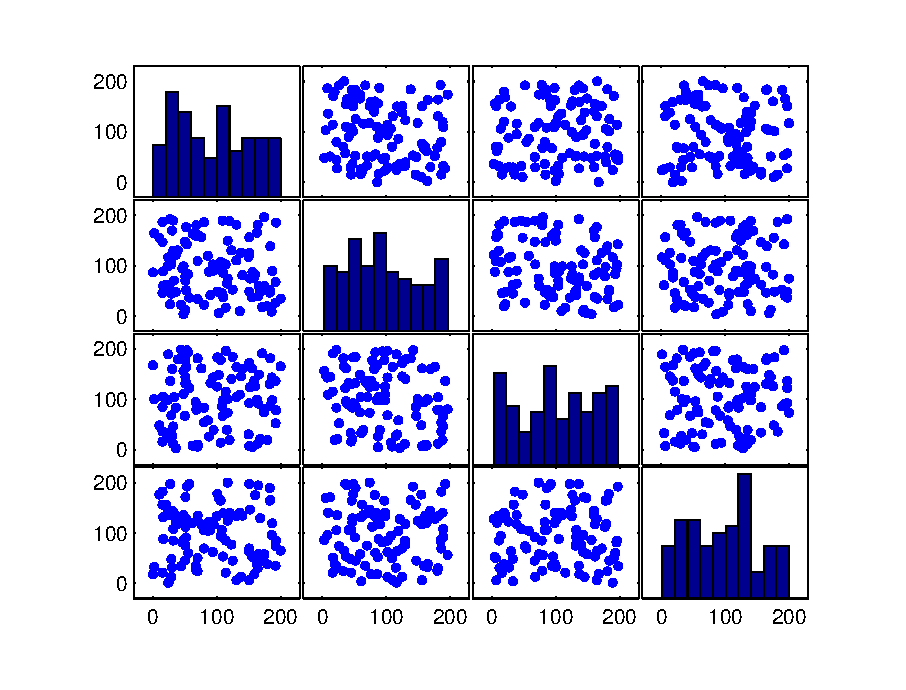
\includegraphics[width=1\textwidth]{rinitcov}
%\end{figure}
%\begin{figure}
%\includegraphics[width=1\textwidth]{rol30cov}
%\end{figure}
%\begin{figure}
%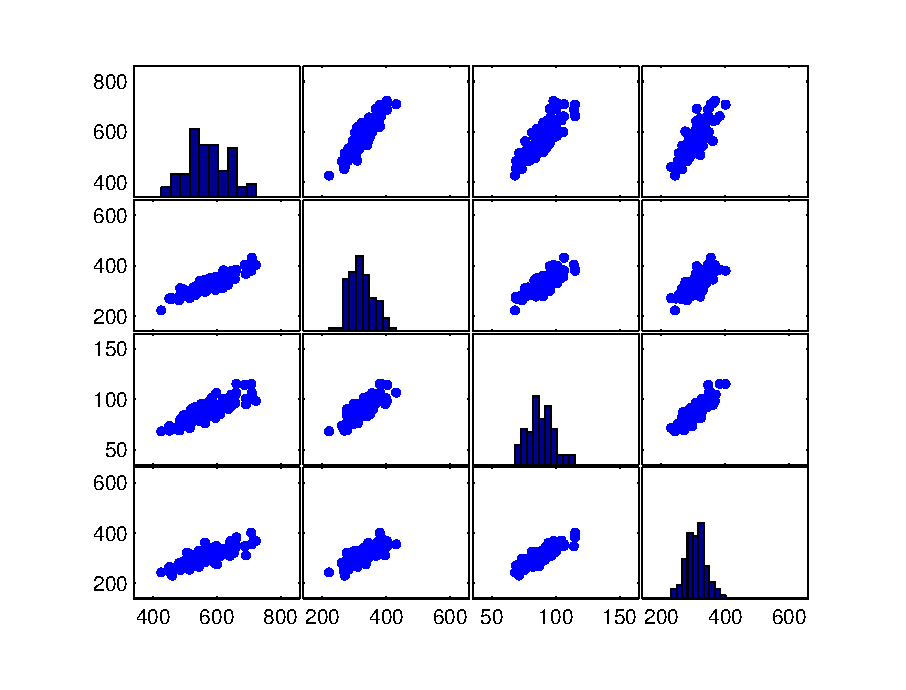
\includegraphics[width=1\textwidth]{rkf30cov}
%\end{figure}

\bibliographystyle{plainnat}
\bibliography{project}
\end{document}
